\documentclass[a5paper, 10pt]{tekst}

\usepackage{titlesec}
\usepackage{indentfirst}

\begin{document}
	\thispagestyle{empty}
	\onehalfspacing
	\titleformat*{\section}{\sffamily\bfseries}
	\sffamily
	
	\begin{center}
		\Huge \p{\f{壁}{かべ}の}\p{\f{穴}{あな}}、\p{\f{第}{だい}}\p{\f{二}{に}\f{話}{わ}}
	\end{center}
	
	\begin{figure}[h]
		\centering
		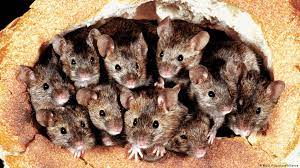
\includegraphics[width=0.5\linewidth]{figures/ねずみ3.jpeg}
	\end{figure}
	
	{\Large\sloppy
		\noindent\ruby{父}{とう}ちゃんは、 \ruby{安全}{あんぜん} で、 もっと \ruby{広}{ひろ}い \ruby{家}{いえ}を \ruby{見}{み}つけなければ いけないと \ruby{言}{い}って、 \ruby{命}{いのち}がけで 3\ruby{泊}{ぱく} \ruby{4日}{よっか}の \ruby{旅}{たび}に \ruby{出}{で}た。 そして、 この \ruby{新}{あたら}しい \ruby{壁}{かべ}の \ruby{穴}{あな}を \ruby{見}{み}つけた らしい。 でも、 \ruby{生}{う}まれたばかりの \ruby{妹}{いもうと}\ruby{達}{たち}が \ruby{自分}{じぶん}で \ruby{歩}{ある}ける ように なるまで、 \ruby{引}{ひ}っ\ruby{越}{こ}しは できなかった。 \ruby{僕}{ぼく}\ruby{達}{たち}は、 その \ruby{間}{あいだ}、 これ \ruby{以上}{いじょう} \ruby{人間}{にんげん}に \ruby{見}{み}られない ように、 とても \ruby{注意深}{ちゅういぶか}く \ruby{過}{す}ごした。 そして、 やっと \ruby{妹}{いもうと}\ruby{達}{たち}が \ruby{歩}{ある}ける ように なって、 \ruby{引}{ひ}っ\ruby{越}{こ}しの \ruby{日}{ひ}が \ruby{決}{き}まったん だ。
		
		\noindent その \ruby{小}{ちい}さな \ruby{妹}{いもうと}\ruby{達}{たち}を \ruby{連}{つ}れて、 3\ruby{軒}{げん}も \ruby{離}{はな}れた この \ruby{新}{あたら}しい \ruby{家}{いえ}に \ruby{引}{ひ}っ\ruby{越}{こ}して \ruby{来}{く}るのは、 \ruby{文字通}{もじどお}り \ruby{命}{いのち}がけ だった。 \ruby{途中}{とちゅう}、 \ruby{猫}{ねこ}を \ruby{飼}{か}っている \ruby{家}{いえ}の \ruby{庭}{にわ}を、 \ruby{通}{とお}らなければ ならなかったから だ。 \ruby{猫}{ねこ}が \ruby{目}{め}を \ruby{覚}{さ}まさない ように、 \ruby{僕}{ぼく}\ruby{達}{たち}は そっと \ruby{息}{いき}を \ruby{殺}{ころ}して \ruby{歩}{ある}いた。 でも、 その \ruby{時}{とき}、 \ruby{猫}{ねこ}が \ruby{片目}{かため}を \ruby{開}{あ}けて こっちを \ruby{見}{み}た。 そして、 \ruby{僕}{ぼく}\ruby{達}{たち}に \ruby{気付}{きづ}いて しまったん だ。 \ruby{僕}{ぼく}は \ruby{心臓}{しんぞう}が \ruby{止}{と}まるかと \ruby{思}{おも}ったよ。 もう、 みんな、 \ruby{死}{し}に \ruby{物狂}{ものぐる}いで \ruby{走}{はし}った。 でも、 \ruby{足}{あし}が \ruby{遅}{おそ}かった 2\ruby{匹}{ひき}の \ruby{妹}{いもうと}\ruby{達}{たち}は、 \ruby{猫}{ねこ}に \ruby{捕}{つか}まって しまった。 あっという\ruby{間}{ま}の \ruby{出来事}{できごと} だった。 それでも、 \ruby{僕}{ぼく}\ruby{達}{たち}は \ruby{止}{と}まる わけには いかなかった。 みんな、 \ruby{悲}{かな}しくて \ruby{泣}{な}きながらも \ruby{必死}{ひっし}で \ruby{走}{はし}った。 だから、 ついに この \ruby{新}{あたら}しい \ruby{家}{いえ}の \ruby{壁}{かべ}の \ruby{穴}{あな}に \ruby{到着}{とうちゃく} できた \ruby{時}{とき}は、 ほっと して \ruby{家族}{かぞく} 4\ruby{匹}{ひき}で \ruby{抱}{だ}き\ruby{合}{あ}った。
		
		\noindent この \ruby{新}{あたら}しい \ruby{家}{いえ}には、 クミコと いう \ruby{小}{ちい}さな \ruby{女}{おんな}の \ruby{子}{こ}が \ruby{住}{す}んでいる。 もちろん、 \ruby{彼女}{かのじょ}の \ruby{両親}{りょうしん}も、 そして、 \ruby{祖父母}{そふぼ}\ruby{達}{たち}も \ruby{一緒}{いっしょ}に \ruby{住}{す}んでいる。 この クミコが、 \ruby{毎日}{まいにち} たくさんの \ruby{食}{た}べ\ruby{物}{もの}を テーブルの \ruby{下}{した}に こぼして くれるん だ。 だから、 「ここに \ruby{引}{ひ}っ\ruby{越}{こ}して \ruby{来}{き}てから、 \ruby{色}{いろ}んな \ruby{食}{た}べ\ruby{物}{もの}を \ruby{食}{た}べられる ように なったわ」 と、 \ruby{僕}{ぼく}の \ruby{両親}{りょうしん}は \ruby{喜}{よろこ}んでいた。
		
	}\clearpage
	\titleformat*{\section}{\rmfamily\bfseries}
	\rmfamily
	
	\section*{Vokabular}
	\begin{multicols}{2}[\centering\textbf{Bitno}]\noindent
		\dictentry{三泊}{さんぱく}{\item tri noći}{brojač}
		\dictentry{旅}{たび}{\item put, putovanje}{imenica, suru-glagol}
		\dictentry{間}{あいだ}{\item sredina, vremenski period}{Imenica, prilog}
		\dictentry{過ごす}{すごす}{\item provoditi (vrijeme)}{glagol(五)}
		\dictentry{決まる}{きまる}{\item biti odlučeno}{glagol(五)}
		\dictentry{連れる}{つれる}{\item povesti sa}{glagol (一)}
		\dictentry{文字通り}{もじどおり}{\item doslovno}{imenica, prilog}
		\dictentry{気付く}{きづく}{\item primijetiti}{glagol(五)}
		\dictentry{心臓}{しんぞう}{\item srce}{imenica}
		\dictentry{あっという間}{あっというま}{\item u trenu / dok kažeš keks}{izraz}
		\dictentry{出来事}{できごと}{\item događaj}{imenica}
		\dictentry{到着}{とうちゃく}{\item dolazak}{imenica, suru-glagol}
	\end{multicols}
	
	\clearpage
	\begin{multicols}{2}[\centering\textbf{Ostalo}]
		\dictentry{第}{だい}{\item prefiks za tvorbu rednih brojeva}{prefiks}
		\dictentry{二話}{にわ}{\item druga epizoda}{brojač}
		\dictentry{父ちゃん}{とうちゃん}{\item tata}{imenica}
		\dictentry{安全}{あんぜん}{\item sigurnost}{imenica, na-pridjev}
		\dictentry{広い}{ひろい}{\item prostrano, široko}{i-pridjev}
		\dictentry{家}{いえ}{\item kuća}{imenica}
		\dictentry{見つける}{みつける}{\item pronaći}{glagol (一)}
		\dictentry{言う}{いう}{\item reći}{glagol(五)}
		\dictentry{命がけ}{いのちがけ}{\item riskirati život}{imenica}
		\dictentry{4日}{よっか}{\item četiri dana}{brojač}
		\dictentry{出る}{でる}{\item izaći}{glagol (一)}
		\dictentry{新しい}{あたらしい}{\item nov}{i-pridjev}
		\dictentry{壁}{かべ}{\item zid}{imenica}
		\dictentry{穴}{あな}{\item rupa}{imenica}
		\dictentry{生まれる}{うまれる}{\item roditi se}{glagol (一)}
		\dictentry{妹}{いもうと}{\item mlađa sestra}{imenica}
		\dictentry{妹達}{いもうとたち}{\item mlađe sestre}{sufiks za množinu}
		\dictentry{自分}{じぶん}{\item ja}{zamjenica}
		\dictentry{歩く}{あるく}{\item hodati}{glagol(五)}
		\dictentry{引っ越す}{ひっこす}{\item preseliti se}{glagol(五)}
		\dictentry{僕}{ぼく}{\item ja, muški}{zamjenica}
		\dictentry{以上}{いじょう}{\item više od}{imenica, prilog}
		\dictentry{人間}{にんげん}{\item čovjek}{imenica}
		\dictentry{見る}{みる}{\item vidjeti}{glagol (一)}
		\dictentry{注意深い}{ちゅういぶかい}{\item oprezan}{i-pridjev}
		\dictentry{小さい}{ちいさい}{\item malen}{i-pridjev}
		\dictentry{3軒}{さんげん}{\item tri kuće}{brojač}
		\dictentry{離れる}{はなれる}{\item odvojiti se}{glagol (一)}
		\dictentry{来る}{くる}{\item doći}{nepravilan glagol}
		\dictentry{途中}{とちゅう}{\item usred}{imenica, prilog}
		\dictentry{猫}{ねこ}{\item mačka}{imenica}
		\dictentry{飼う}{かう}{\item imati (životinju)}{glagol(五)}
		\dictentry{庭}{にわ}{\item vrt}{imenica}
		\dictentry{通る}{とおる}{\item proći kroz}{glagol(五)}
		\dictentry{目を覚ます}{めをさます}{\item probuditi se}{izraz}
		\dictentry{息を殺す}{いきをころす}{\item zadržavati dah}{izraz}
		\dictentry{時}{とき}{\item tren, vrijeme}{imenica, prilog}
		\dictentry{片目}{かため}{\item jedno oko}{imenica}
		\dictentry{開ける}{あける}{\item otvoriti}{glagol(一)}
		\dictentry{止まる}{とまる}{\item stati}{glagol(五)}
		\dictentry{思う}{おもう}{\item misliti}{glagol(五)}
		\dictentry{死に物狂い}{しにものぐるい}{\item očajnički}{izraz}
		\dictentry{走る}{はしる}{\item trčati}{glagol(五)}
		\dictentry{足}{あし}{\item noga}{imenica}
		\dictentry{遅い}{おそい}{\item spor}{i-pridjev}
		\dictentry{二匹}{にひき}{\item dvije male životinje}{brojač}
		\dictentry{捕まる}{つかまる}{\item biti uhvaćen}{glagol(五)}
		\dictentry{悲しい}{かなしい}{\item tužan}{i-pridjev}
		\dictentry{泣く}{なく}{\item plakati}{glagol(五)}
		\dictentry{必死}{ひっし}{\item očajno}{na-pridjev, no-pridjev}
	\end{multicols}
	
	\clearpage
	
	\section*{Domaća zadaća}
	\begin{enumerate}
		\item Napišite kratku priču ili par rečenica koristeći riječi iz kutije ispod.
		Rečenice ili tekst ne moraju nužno biti vezane uz sam tekst.
		\begin{center}
			\vspace{0.5em}
			\fbox{旅 ・ 過ごす ・ 心臓 ・ 出来事 ・ 到着}\vspace{1.4em}
			\rule{\linewidth}{0.5pt}\\[0.6em]
			\rule{\linewidth}{0.5pt}\\[0.6em]
			\rule{\linewidth}{0.5pt}\\[0.6em]
			\rule{\linewidth}{0.5pt}\\[0.6em]
			\rule{\linewidth}{0.5pt}\\[0.6em]
			\rule{\linewidth}{0.5pt}\\[0.6em]
			\rule{\linewidth}{0.5pt}
		\end{center}
		
		\item Odgovorite na pitanja:
		\begin{enumerate}[label=(\roman*)]
			\raggedright
			\item\vspace{0.5em}\p{\f{父}{ちち}ちゃんは}\p{\f{新}{あたら}しい}\p{\f{壁}{かべ}の}\p{\f{穴}{あな}を}\p{\f{見}{み}つける}\p{ために}\p{何を}\p{しましたか?}
			\rule{\linewidth}{0.5pt}\\[0.6em]
			\rule{\linewidth}{0.5pt}
			\item\vspace{0.5em}\p{何で}\p{今}\p{すぐに}\p{\f{引っ越}{ひっこ}し}\p{できませんでした?}
			\rule{\linewidth}{0.5pt}\\[0.6em]
			\rule{\linewidth}{0.5pt}
			\item\vspace{0.5em}\p{\f{引っ越}{ひっこ}しの}\p{\f{途中}{とちゅう}で}\p{何が}\p{ありました?}
			\rule{\linewidth}{0.5pt}\\[0.6em]
			\rule{\linewidth}{0.5pt}
			\item\vspace{0.5em}\p{\f{新}{あたら}しい}\p{\f{壁}{かべ}の}\p{\f{穴}{あな}は}\p{前のと}\p{どう}\p{\f{違}{ちが}うのですか?}
			\rule{\linewidth}{0.5pt}\\[0.6em]
			\rule{\linewidth}{0.5pt}
			\item\vspace{0.5em}\p{\f{語り手}{かたりて}の}\p{\f{両親}{りょうしん}は}\p{何で}\p{\f{喜}{よろこ}んで}\p{いますか?}
			\rule{\linewidth}{0.5pt}\\[0.6em]
			\rule{\linewidth}{0.5pt}
		\end{enumerate}		
		\item Nadopunite sljedeće rečenice riječima iz kutije ispod:
		\begin{center}
			\choicebox{泊 ・ 旅 ・ 間 ・ 過ごした ・ 決まった ・ 連れて ・ 文字通り\\気付きませんでした ・ 心臓 ・ あっという間 ・ 出来事 ・ 到着}
		\end{center}
		\begin{enumerate}[label=(\roman*)]
			\raggedright
			
			\vspace{0.5em}\item \p{\f{私}{わたくし}は}\p{\f{名古屋}{なごや}に}\p{一\ansline{}}\p{\f{旅行}{りょこう}を}\p{する}\p{\f{計画}{けいかく}を}\p{して}\p{いる。}
			\item \p{\ansline{}に}\p{\f{行}{い}く}\p{ときは}\p{ブラシを}\p{\f{持}{も}って}\p{いくのは}\p{\f{当然}{とうぜん}だ。}
			\item \p{\f{川}{がわ}と}\p{\f{丘}{おか}の\ansline{}}\p{にむらが}\p{ある。}
			\item \p{\f{石子}{いしこ}は}\p{「\f{昨}{さく}}\p{\f{日本}{にっぽん}\f{屋}{や}で\ansline{}}\p{\f{数}{すう}}\p{\f{時間}{じかん}は}\p{\f{幻想}{げんそう}\f{的}{てき}でした」と}\p{\f{金魚}{きんぎょ}の}\p{\f{幸子}{さちこ}ちゃんに}\p{話しました。}
			\item \p{\f{去年}{きょねん}}\p{\f{賛子}{あきこ}の}\p{\f{村}{むら}で}\p{\f{近郊}{きんこう}の}\p{\f{森}{もり}}\p{\f{全部}{ぜんぶ}を}\p{でかい}\p{\f{壁}{かべ}を}\p{\f{作}{つく}る}\p{ために}\p{\f{使}{つか}うと\ansline{}から、}\p{\f{賛子}{あきこ}は}\p{今でも}\p{それを}\p{\f{止}{と}めようと}\p{して}\p{いる。}
			\item \p{\f{花子}{はなご}ちゃん、}\p{\f{武}{たけし}\f{君}{くん}を\ansline{}}\p{ビーチに}\p{\f{来}{き}てね、}\p{スイカ}\p{\f{割}{わり}}\p{するから。}
			\item \p{\f{愛子}{あいこ}は}\p{\f{先生}{せんせい}の\ansline{}}\p{\f{数学}{すうがく}の}\p{\f{問題}{もんだい}を}\p{\f{解}{と}いたけど}\p{\f{何}{なん}}\p{\f{回}{かい}}\p{\f{解}{と}いても}\p{\f{答}{こた}えは}\p{\f{正}{ただ}しく}\p{なかった。}
			\item \p{\f{腕}{うで}を}\p{\f{蚊}{か}に}\p{\f{刺}{さ}されて}\p{いるのに\ansline{}。}
			\item \p{\f{人}{ひと}ごみに}\p{そんなに}\p{\f{長}{なが}く}\p{いるのは\ansline{}に}\p{\f{悪}{わる}い。}
			\item \p{一}\p{\f{週間}{しゅうかん}}\p{\f{後山}{あとやま}を}\p{\f{登}{のぼ}りに}\p{\f{行}{い}ったけど\ansline{}に}\p{\f{疲}{つか}れて}\p{五}\p{\f{時間}{じかん}も}\p{かかったのさ。}
			\item \p{\f{武}{たけし}\f{君}{くん}は}\p{「\f{僕}{ぼく}は}\p{その\ansline{}とは}\p{\f{何}{なん}の}\p{\f{関係}{かんけい}も}\p{ない」と}\p{\f{言}{い}ったけど、}\p{\f{誰}{だれ}も}\p{\f{信}{しん}じなかった。}
			\item \p{\f{消防}{しょうぼう}\f{車}{しゃ}が\ansline{}}\p{した}\p{時に}\p{ラブ}\p{ホテルは}\p{すでに}\p{\f{燃}{も}え}\p{つくした。}
		\end{enumerate}
	\end{enumerate}
\end{document}